% Presentation-only derivative; scripts/build_appendix_compact_tables_20261106.py
\begin{figure}[!htbp]
\centering
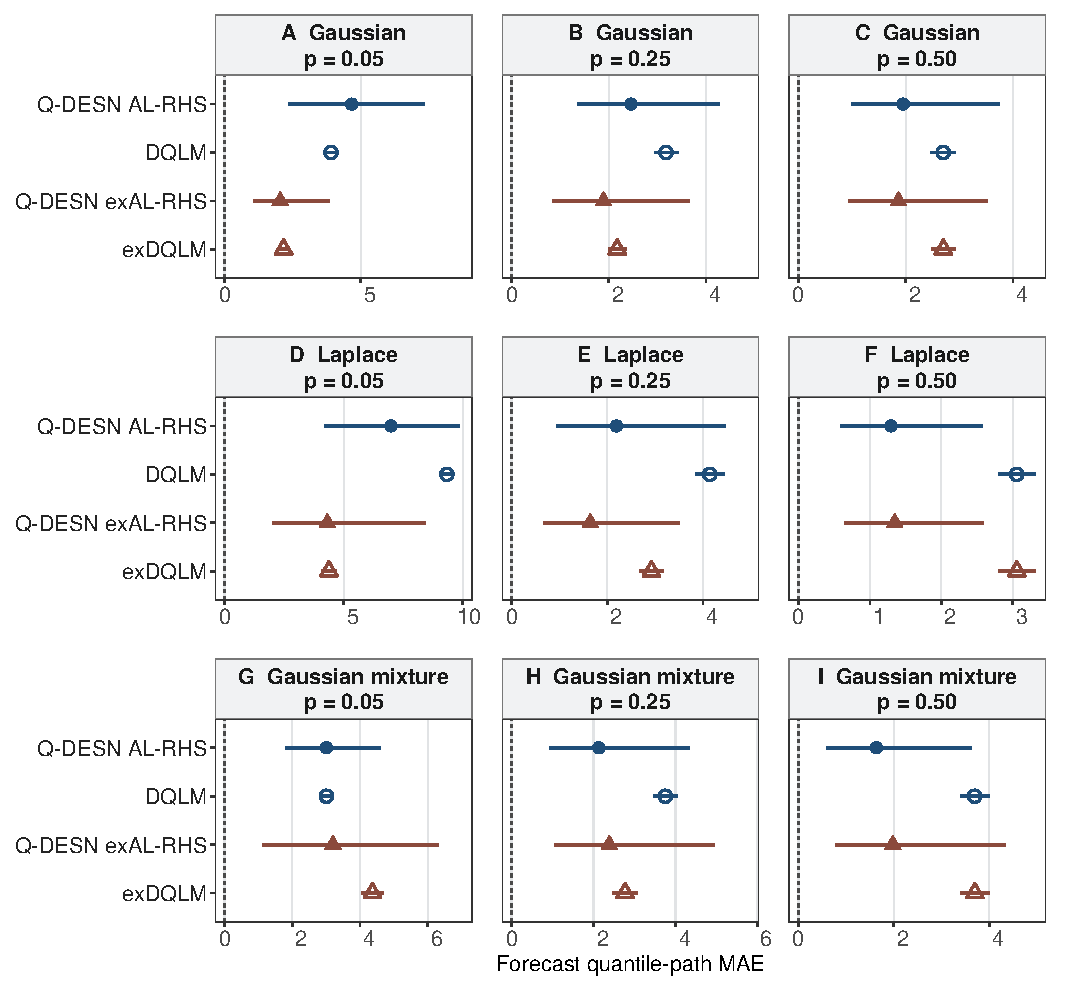
\includegraphics[width=0.98\textwidth]{figures/independent_simulation/independent_train500_eval300_mcmc_forecast_mae_v1.pdf}
\caption{MCMC forecast quantile-path MAE over 300 targets (10 origins). Points and equal-tailed 95\% intervals summarize draw-wise aggregate recovery error; lower is better. Navy circles denote AL and muted-brick triangles exAL; filled symbols denote Q--DESN and open symbols dynamic linear comparators. Panels identify family and level. The dashed line marks exact recovery. Corresponding 500-target panels use the same horizontal limits; intervals depend on the model-specific draw construction.}
\figalt{Nine panels compare four models using mean forecast quantile-path MAE and 95 percent intervals over 300 scored targets.}
\label{fig:simulation-500obs-mcmc-forecast-mae-intervals}
\end{figure}
